\documentclass{unswmaths}
\usepackage{shortcuts}
\usepackage[all]{xy}
\usepackage{csquotes}
\usepackage{color}
\usepackage[square,numbers]{natbib}
\usepackage{tikz}

\begin{document}

\subject{MATH5425 - Graph Theory}
\author{Edward McDonald}
\title{Assignment 1}
\studentno{z3375335}


\setlength\parindent{0pt}


\newcommand{\bd}{\boldsymbol{d}}

\unswtitle{}

\section*{Question 1}
For this question, $G$ is a graph with $n$ vertices.
\begin{proposition}[Part (a)]
\label{1a}
    Suppose that $G$ has at least $n$ edges. Then $G$ contains a cycle.
\end{proposition}
\begin{proof}
    Suppose that $G$ has $k$ connected components, $G_1,\ldots,G_k$.
    There must exist a connected component $G_j$
    with $|E(G_j)| \geq |V(G_j)|$, since otherwise we
    would have $|E(G)| < |V(G)|$, but we are assuming
    that $|E(G)| \geq n$. 
    
    Let $G_j$ be a connected component with $|E(G_j)| \geq |V(G_j)|$.
    We will show that $G_j$ contains a cycle. If $G_j$ contains
    no cycle, then $G_j$ is a tree by definition. However by Corollary
    $1.5.3$ in the course notes, this can only be true if $|E(G_j)| = |V(G_j)|-1$.
    But this contradicts $|E(G_j)| \geq |V(G_j)|$. Hence $G_j$ contains a cycle.
\end{proof}

\begin{proposition}[Part (b)]
\label{1b}
    Suppose that $G$ has strictly more than $n$ edges. Then $G$ contains
    two distinct (not necessarily disjoint) cycles.
\end{proposition}
\begin{proof}
    Let $e \in E(G)$. Then $G - e$ has at least $n$ edges, so by Proposition \ref{1a}
    $G-e$ contains a cycle. Call such a cycle $C_1$.
    
    Now choose $f \in E(C)$. Again by proposition \ref{1a}, $G-f$ contains
    a cycle, call it $C_2$.
    
    Hence $C_1$ and $C_2$ are two cycles in $G$, and since $f \in C_1$
    and $f \notin C_2$, the cycles are distinct.
\end{proof}

\begin{proposition}[Part (c)]
    Suppose that $G$ has minimum degree $\delta(G) \geq 3$. Then $G$ contains
    a cycle of even length.
\end{proposition}
\begin{proof}
    Observe that $G$ always contains at least one cycle, since
    by the handshaking lemma,
    \begin{equation}
        2|E(G)| = \sum_{v \in V(G)} d_G(v) \geq 3|V(G)|.
    \end{equation}
    Hence $E(G) \geq V(G)$, so by Proposition \ref{1a} $G$ contains a cycle.
    
    We will perform a proof by contradiction. We will assume that $G$ contains only
    odd cycles, then construct a cycle of even length.
    
    Assume that $G$ contains only odd cycles.
    
    First suppose that $G$ is connected. Let $T$ be a spanning tree for $G$,
    and let $w$ be a leaf of $T$ connected to the edge $t \in E(T)$. Hence $d_T(w) = 1$ but $d_G(v) \geq 3$,
    so there exist two distinct edges, $e,f \in E(G)$ with endpoints at $w$
    not contained in $T$.
    
    Now, since a tree is maximally acyclic, $T+e$ contains a cycle $C_1$
    and $T+f$ contains a cycle $C_2$. We must have $t$ as an edge of $C_1$
    and $C_2$, since $C_1$ must pass through $e$, and hence through $t$
    since $d_{T+e}(w) = 2$,
    similarly $C_2$ must pass through $t$. By assumption $C_1$
    and $C_2$ have odd length.
    
    Suppose that $C_1$ and $C_2$ contain $k$ common edges. 
    We must have $k \geq 1$ since $t$ is common.
    Consider the cycle $C$ obtained by joining together $C_1$ and $C_2$, and
    removing the common edges this is possible since $k \geq 1$. Hence $|E(C)| = |E(C_1)|+|E(C_2)|-2k$.
    But then $|E(C)|$ is even, since by assumption $|E(C_1)|$ and $|E(C_2)|$
    are odd.
    
    Hence $G$ contains an even cycle when $G$ is connected.
    
    If $G$ is not connected, then each connected component $H$
    satisfies $\delta(H) \geq 3$, so we may run the above argument
    to show that $H$ has a cycle of even length, so hence $G$
    has a cycle of even length.
   
\end{proof}

\section*{Question 2}
We shall say that a graph $G$ on $n$ vertices has degree sequence $\bd = (d_1,d_2,\ldots,d_n)$
if $\bd$ is a nondecreasing sequence and the degrees
of the vertices of $G$ when arranged in nondecreasing order are the entries of $\bd$.
We consider the following condition:
\begin{equation}\tag{*}
\label{star}
\sum_{i=1}^n d_i = 2n-2.
\end{equation}

\begin{proposition}[Part (a)]
\label{2a}
    Suppose that $T$ on $n$ vertices with degree sequence $\bd$.
    Then $\bd$ satisfies (\ref{star}).
\end{proposition}
\begin{proof}
    By Corollary 1.5.3 in the course notes, $T$ has $n-1$ edges.
    Hence by the handshaking lemma,
    \begin{equation}
        \sum_{i=1}^n d_i = 2|E(T)| = 2(n-1) = 2n-2.
    \end{equation}
    So (\ref{star}) holds.
\end{proof} 
\begin{proposition}[Part (b)]
\label{2b}
    Now suppose that $n = 2$, and $\bd$ is a sequence such that
    (\ref{star}) holds. Then there exists a tree $T$ with degree
    sequence $\bd$.
\end{proposition}
\begin{proof}
    If (\ref{star}) holds, then $d_1+d_2 = 2(2)-2 = 2$. Hence
    we can choose $T$ to be the unique tree on two vertices. Then
    we have $d_1 = d_2 = 1$.
\end{proof}
\begin{proposition}[Part (c)]
\label{2c}
    Now let $n \geq 3$, and let $\bd$ be a sequence such that (\ref{star}) holds.
    Let $\delta = d_1$ and $\Delta = d_n$ be the minimum and maximum entries of $\bd$
    respectively. Then,
    \begin{enumerate}
        \item{} $\delta = 1$ and $\Delta \geq 2$.
        \item{} There exists a tree $T$ with degree sequence $\bd$.
    \end{enumerate}
\end{proposition}
\begin{proof}
    First we prove $(1)$. Suppose that $\delta \geq 2$. This means that
    \begin{equation}
        \sum_{i=1}^n d_i \geq 2n.
    \end{equation}
    But then $2n-2 \geq 2n$, which is impossible. Now if we assume that $\Delta < 2$,
    then we must have $\Delta = 1$, so $\bd = (1,1,\ldots,1)$. Thus,
    \begin{equation}
        n = \sum_{i=1}^n d_i = 2n-2.
    \end{equation}
    But then $n = 2$, which is impossible since $n \geq 3$ by assumption.
    
    Now we prove $(2)$ by induction. Suppose that for all $k < n$, we know
    that for any degree sequence $(d_1,d_2,\ldots,d_k)$ with $\sum_{i=1}^k d_i = 2k-2$
    there exists a tree on $k$ vertices with degree sequence $k$.
    
    Now let $\bd = (d_1,\ldots,d_n)$ be a sequence satisfying (\ref{star}).
    
    Let
    \begin{equation}
        q = \min\{ j \; d_j > 1\}.
    \end{equation}
%    We know that $q > 1$, since we proved that $\Delta \geq 2$. 
%    Now if $q = n$, then the sequence must be $\bd = (1,1,\ldots,2)$, so
%    it must be $\bd = (1,1,2)$. In this case, choose $T$ to be the tree:
%    \begin{center}
%        \begin{tikzpicture}
%            \draw [fill] (0,0) circle (0.1);
%            \draw [fill] (0,1) circle (0.1);
%            \draw [fill] (1,0) circle (0.1);
%            
%            \draw [-] (0,0) -- (0,1);
%            \draw [-] (0,0) -- (1,0);
%        \end{tikzpicture}
%    \end{center}
%    Then $T$ has degree sequence $(1,1,2)$.
    
    Consider
    the sequence of $n-1$ numbers,
    \begin{equation}
        \tilde{\bd} = (d_2\ldots,d_q-1,\ldots,d_n).
    \end{equation}
    if $q < n$, and $\tilde{\bd} = (d_2,\ldots,d_n-1)$ if $q = n$.
    Then we can see that $\bd$ is a sequence satisfying (\ref{star}), since
    for $q < n$:
    \begin{equation}
        d_2+\cdots+(d_q-1) + \cdots + d_n = 2n-2-1-d_n = 2n-4 = 2(n-1) - 2.
    \end{equation}
    
    If $q = n$, then we must have $\bd = (1,1,\ldots,1,d_n)$. Hence $n-1+d_n = 2n-2$, so
    $d_n = n-1$, and 
    \begin{equation}
        d_2 + \cdots + d_n-1 = \underbrace{1+\cdots+1}_{n-2\text{ times}}+d_n-1 = 2(n-2)  = 2(n-1)-2.
    \end{equation}
    Hence, there exists a tree with degree sequence $\tilde{\bd}$ by our inductive
    hypothesis. Let $T$ be such a tree, and let $v$ be a vertex
    with degree $d_q - 1$. 
    
    Consider the tree $F$ obtained by joining a new leaf to $v$. Then $F$
    has $n$ vertices, and has degree sequence $(1,d_2,\ldots,d_n) = \bd$.
    Thus the assertion is proved by induction since by Proposition \ref{2b} it is true for $n=2$.
\end{proof}
\begin{proposition}[Part (d)]
\label{2d}
    There exist two non-isomorphic trees with identical degree sequence.
\end{proposition}
\begin{proof}
    Consider the following two trees.
    $T_1$:
    \begin{center}
        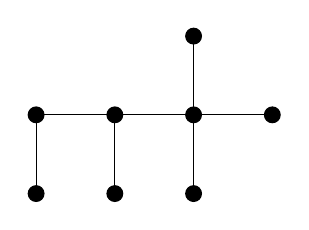
\begin{tikzpicture}
            \draw [fill] (0,0) circle (0.1);
            \draw [fill] (0,1) circle (0.1);
            \draw [fill] (1,0) circle (0.1);
            \draw [fill] (1,1) circle (0.1);
            \draw [fill] (2,0) circle (0.1);
            \draw [fill] (2,1) circle (0.1);
            \draw [fill] (2,2) circle (0.1);
            \draw [fill] (3,1) circle (0.1);
            
            \draw [-] (0,0) -- (0,1);
            \draw [-] (1,0) -- (1,1);
            \draw [-] (2,0) -- (2,1);
            \draw [-] (0,1) -- (1,1);
            \draw [-] (1,1) -- (2,1);
            
            \draw [-] (2,1) -- (2,2);
            \draw [-] (2,1) -- (3,1);
        \end{tikzpicture}
    \end{center}
    
    and $T_2$:
    \begin{center}
        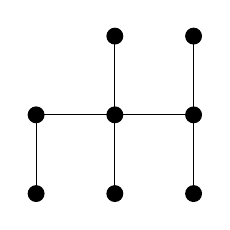
\begin{tikzpicture}
            \draw [fill] (0,0) circle (0.1);
            \draw [fill] (0,1) circle (0.1);
            \draw [fill] (1,0) circle (0.1);
            \draw [fill] (1,1) circle (0.1);
            \draw [fill] (2,0) circle (0.1);
            \draw [fill] (2,1) circle (0.1);
            \draw [fill] (2,2) circle (0.1);
            \draw [fill] (1,2) circle (0.1);
            
            \draw [-] (0,0) -- (0,1);
            \draw [-] (1,0) -- (1,1);
            \draw [-] (2,0) -- (2,1);
            \draw [-] (0,1) -- (1,1);
            \draw [-] (1,1) -- (2,1);
            
            \draw [-] (1,1) -- (1,2);
            \draw [-] (2,1) -- (2,2);
        \end{tikzpicture}
    \end{center}
    
    We can see that $T_1$ and $T_2$ both have degree sequence $(1,1,1,1,1,2,3,4)$,
    but they are not isomorphic, since $T_1$ has a vertex of degree $4$ attached to $3$
    leaves, but $T_2$ only has a vertex of degree $4$ attached to $2$ leaves.
\end{proof}

\section*{Question 3}
For this question, we let $G$ be the following graph on 10 vertices:
\begin{center}
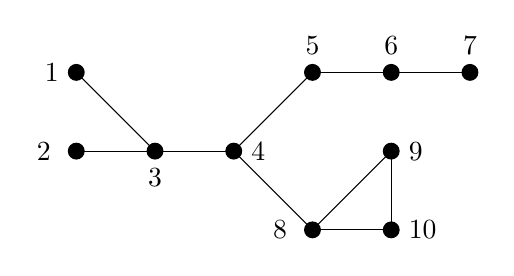
\begin{tikzpicture}
\draw [-] (4,3) -- (5,3);
\draw [-] (3,3) -- (4,3);
\draw [-] (4,3) -- (3,4);
\draw [-] (4,3) -- (5,3);
\draw [-] (5,3) -- (6,4);
\draw [-] (6,4) -- (7,4);
\draw [-] (7,4) -- (8,4);
\draw [-] (5,3) -- (6,2);
\draw [-] (6,2) -- (7,3);
\draw [-] (6,2) -- (7,2);
\draw [-] (7,2) -- (7,3);
\draw [fill] (3,3) circle (0.1);
\draw [fill] (3,4) circle (0.1);
\draw [fill] (4,3) circle (0.1);
\draw [fill] (5,3) circle (0.1);
\draw [fill] (6,2) circle (0.1);
\draw [fill] (6,4) circle (0.1);
\draw [fill] (7,2) circle (0.1);
\draw [fill] (7,3) circle (0.1);
\draw [fill] (7,4) circle (0.1);
\draw [fill] (8,4) circle (0.1);
\node [left] at (2.9,4) {$1$};
\node [left] at (2.8,3) {$2$};
\node [below] at (4,2.9) {$3$};
\node [right] at (5.1,3) {$4$};
\node [above] at (6,4.1) {$5$};
\node [above] at (7,4.1) {$6$};
\node [above] at (8,4.1) {$7$};
\node [left] at (5.8,2) {$8$};
\node [right] at (7.1,3) {$9$};
\node [right] at (7.1,2) {$10$};
\end{tikzpicture}
\end{center}
\begin{proposition}[Part (a)]
\label{3a}
    There is no perfect matching of $G$.
\end{proposition}
\begin{proof}
    By Tutte's theorem (Theorem 2.1.1 in the course notes), it suffices to find
    $S \subseteq V(G)$ such that the number of connected components of $G-S$ with
    an odd number of vertices, $q(G-S)$
    exceeds $|S|$.
    
    Take $S = \{4\}$. Then the connected components of $G-S$ have vertices $\{1,2,3\}$,
    $\{5,6,7\}$ and $\{8,9,10\}$. Hence $q(G-S) = 3$. But $|S| = 1$, so $q(G-S) > |S|$.
    Thus there is no perfect matching of $G$.
\end{proof}
\begin{proposition}[Part (b)]
\label{3b}
    A maximum matching of $G$ is:
    \begin{equation}
        M = \{ 23,45,67,89\}.
    \end{equation}
\end{proposition}
\begin{proof}
    It is clear from the picture that $M$ is a matching. Since $M$ covers $8$
    vertices, and there is no matching of $G$ with 10 vertices by Proposition \ref{3a}, 
    and a matching must cover an even number of vertices, we conclude that 
    $M$ is maximum.
\end{proof} 


\section*{Question 4}
\begin{proposition}[Part (a)]
\label{4a}
    Let $G$ be a graph on $2r$ vertices, with minimum degree $\delta(G) \geq r$
    with $r \geq 1$. Then $G$ has a perfect matching.
\end{proposition}
\begin{proof}
    By Dirac's theorem (Theorem 10.1.1 in the course notes), $G$ has a Hamilton cycle.
    Label the vertices of $G$ as $v_1,v_2,\ldots,v_{2r}$ so that the cycle
    passes through $v_1v_2\cdots v_{2r}$. Now match up vertices
    according to the cyclic order, $\{v_1,v_2\},\{v_3,v_4\},\ldots,\{v_{2r-1},v_{2r}\}$.
    This is possible since $2r$ is even. Hence $G$ has a perfect matching.
\end{proof}
For the remainder of this question, $G$ is a graph on $n$ vertices with minimum
degree $\delta(G) \geq 1$, and $\Delta := \Delta(G)$ is the maximum degree.
Let $F$ be a maximum matching of $G$, and let $\nu := \nu(G) = |F|$ be the size of
a maximum matching in $G$. Recall that we say that a vertex $x$ of $G$
is covered by $F$ if $x$ is an endpoint of an edge in $F$.
\begin{proposition}[Part (b) i]
\label{4b1}
    Let $x$ be a vertex not covered by $F$. Then every neighbour of $x$
    is covered by $F$.
\end{proposition}
\begin{proof}
    If $x$ has a neighbour $y$ not covered by $F$, then $F\cup\{xy\}$
    is a matching strictly larger than $F$, which contradicts the assumption
    that $F$ is maximum. Hence every neighbour of $x$ is covered by $F$.
\end{proof}
\begin{proposition}[Part (b) ii]
\label{4b2}
    Let $x,y$ be two distinct vertices not covered by $F$, and $a,b \in V(G)$.
    If $xa,yb \in E(G)$, then $ab \notin F$.
\end{proposition}
\begin{proof}
    If $a$ and $b$ are not distinct, then $ab \notin F$. So assume that $a \neq b$.
    Suppose that $xa,yb \in E(G)$, and $ab \in F$. Then consider
    the set $F' = (F \setminus \{ab\})\cup \{xa,yb\}$. Then $F'$ is a matching
    strictly larger than $F$, contradicting the assumption that $F$ is maximum.
\end{proof} 

\begin{proposition}[Part (b) iii]
\label{4b3}
The number of vertices of $G$ not covered by $F$ is at most $(\Delta-1)\nu$.
\end{proposition}
\begin{proof}
    Let $v_1,v_2,\ldots,v_\nu$ be a set of representative vertices
    of each edge in $F$. That is, for each $e \in F$ there
    is exactly one $k$ so that $v_k$ is incident on $e$. 
    Now, for each $1 \leq k \leq \nu$, $v_k$ has at most $\Delta - 1$
    unmatched neighbours since it has at most $\Delta$ neighbours in total
    and it connected to at least one matched vertex. This means that there cannot be more
    than $\nu(\Delta-1)$ unmatched vertices. 
\end{proof}
\begin{proposition}[Part (b) iv]
\label{4b4}
We have $\nu \geq n/(\Delta+1)$.
\end{proposition}
\begin{proof}
    Let $k$ be the number of vertices of $G$ not covered by $F$.
    However each edge of $F$ connects to two unique vertices, so the number
    of edges covered by $F$ is $2\nu$.
    Thus
    $n = k+2\nu$. But by Proposition \ref{4b3}, $k \leq (\Delta-1)\nu$.
    Hence,
    \begin{align}
        n &= k+2\nu\\
        &\leq (\Delta-1)\nu+2\nu\\
        &= (\Delta+1)\nu.
    \end{align}
    So $\nu \geq n/(\Delta+1)$.
\end{proof}

\begin{remark}
    The above estimate is sharp. Consider a triangle graph. 
    In this case, $n = 3$, $\Delta = 2$ and $\nu = 1$.
\end{remark}


\section*{Question 5}
For this question, $G$ is a 2-edge connected graph. That is, $G$
is connected and for any $e \in E(G)$, $G-e$ is connected. 
We define a relation $\sim$ on $E(G)$ as follows: $e \sim f$ if and only
if $e = f$ or $G - \{e,f\}$ is disconnected.
\begin{proposition}[Part (a)]
\label{5a}
    Let $e,f \in E(G)$ be such that every cycle containing $e$ contains $f$
    and vice versa.
    Then $e \sim f$.
\end{proposition}
\begin{proof}    
    We prove the contrapositive: we show that if $e \nsim f$, then there
    is a cycle containing $e$ but not $f$.
    
    Assume that $e \nsim f$. Then $e$ and $f$ are distinct, and $G - \{e,f\}$
    is connected. Let $e = xy$. Then there is a path $P$ joining $x$ and $y$
    in $G - \{e,f\}$. Hence $P+e$ is a cycle in $G$ containing $e$ but not $f$. 
    
    Hence if every cycle containing $e$ contains $f$, then $e \sim f$.
    Thus \emph{a forteriori}, if every cycle containing $e$ contains $f$
    and vice versa, $e \sim f$.
\end{proof}

\begin{proposition}[Part (b)]
\label{5b}
Suppose we have $e,f \in E(G)$ with $e \sim f$. Then every cycle which contains $e$
also contains $f$.
\end{proposition}
\begin{proof}
    If $e = f$ the result is trivial, so we consider $e \neq f$. 
    
    Hence, $G - \{e,f\}$ is disconnected, but since $G$ is $2$-edge connected,
    we have that $G - e$ and $G-f$ are connected. 
    
    Assume, to find a contradiction, that $C$ be a cycle in $G$ which contains $e$ but not $f$. Let $a,b \in V(G)$
    be two vertices which are disconnected in $G-\{e,f\}$. Let $P$ be a path joining
    $a$ and $b$ in $G-f$. Hence $P$ must pass through $e$.
    
    But if $P$ passes through $e$, then this is a contradiction since we can adjoin $C-e$
    to the path $P-e$ to get a path joining $a$ and $b$ in $G-\{e,f\}$. 
    
    Thus, every cycle containing $e$ must contain $f$.
\end{proof}

\begin{proposition}[Part (c)]
\label{5c}
    $\sim$ is an equivalence relation on $E(G)$, and the equivalence classes
    of $\sim$ are subsets of cycles of $G$.
\end{proposition}
\begin{proof}
    We must prove that $\sim$ is reflexive, symmetric and transitive.
    
    We immediately get that for any edge $e$, $e \sim e$ since $e = e$.
    
    Now if $e \sim f$, then $e = f$ or $G - \{e,f\}$ is disconnected. 
    But this holds true if and only if $f = e$ and $G - \{f,e\}$ is connected.
    Hence $f \sim e$ so $\sim$ is symmetric.
    
    Now we prove that $\sim$ is transitive. Let $e,f,g$ be edges with $e \sim f$
    and $f \sim g$. Then by Proposition \ref{5b}, every cycle which contains $e$
    also contains $f$, and every cycle which contains $f$ contains $g$.
    Hence every cycle containing $e$ also contains $g$. Hence, by Proposition \ref{5a}
    we conclude that $e \sim f$.    
    
    Let $e$ is an edge, and $[e]_\sim$ is the equivalence class
    of $\sim$ containing $e$. 
    $e$ must be contained in a cycle, since otherwise $G-e$ is disconnected, which
    contradicts $2$-edge-connectivity.
    
    Let $C$ be a cycle containing $e$. Then every 
    element of $[e]_\sim$ is contained in $\sim$ by Proposition \ref{5b}. 
    Thus $[e]_\sim \subseteq E(C)$.
\end{proof}

\begin{proposition}[Part (d)]
\label{5d}
    Let $P \subseteq E(G)$ be an equivalence class of $\sim$. Then every connected
    component of $G-P$ with at least two vertices is $2$-edge-connected.
\end{proposition}
\begin{proof}
    Let $H$ be a connected component of $G-P$ with at least two vertices, and 
    let $x,y \in V(H)$. It is required to prove that $H - xy$ is connected. 
    In other words, we must prove that $H$ contains a cycle containing $xy$. 
    Note that there exists a cycle containing $xy$ in $G$ since $G$ is $2$-edge-connected.
    
    We now show that there exists a cycle containing $xy$ in $G$ which is disjoint
    from every element of $P$. 
    
    Suppose that $C$ is a cycle in $G$ containing $xy$ which also contains $e \in P$.
    But then since $C$ is a cycle containing $e$, it must also contain all $f$
    such that $f \sim e$. Hence if $C$ is a cycle containing some element of $P$,
    it must contain all elements of $P$. So it suffices to show that there is a cycle
    containing $xy$ which does not contain a particular element of $P$.
    
    Let $e \in P$, then since $e \nsim xy$, by Proposition \ref{5a}, there is a cycle
    containing $xy$ but not $e$.
    
    Hence, there is a cycle $C$ containing $xy$ disjoint from $P$, so $C$ is a cycle
    in $G-P$ containing $xy$. Hence, $H$ contains a cycle containing $xy$. Therefore,
    $H$ is $2$-edge-connected.
\end{proof}


\end{document}
